% Chapter Template

\chapter{Results} % Main chapter title

\section{Qualitative and quantitive descriptions of slow waves}
\begin{figure}[!htb]
\centering
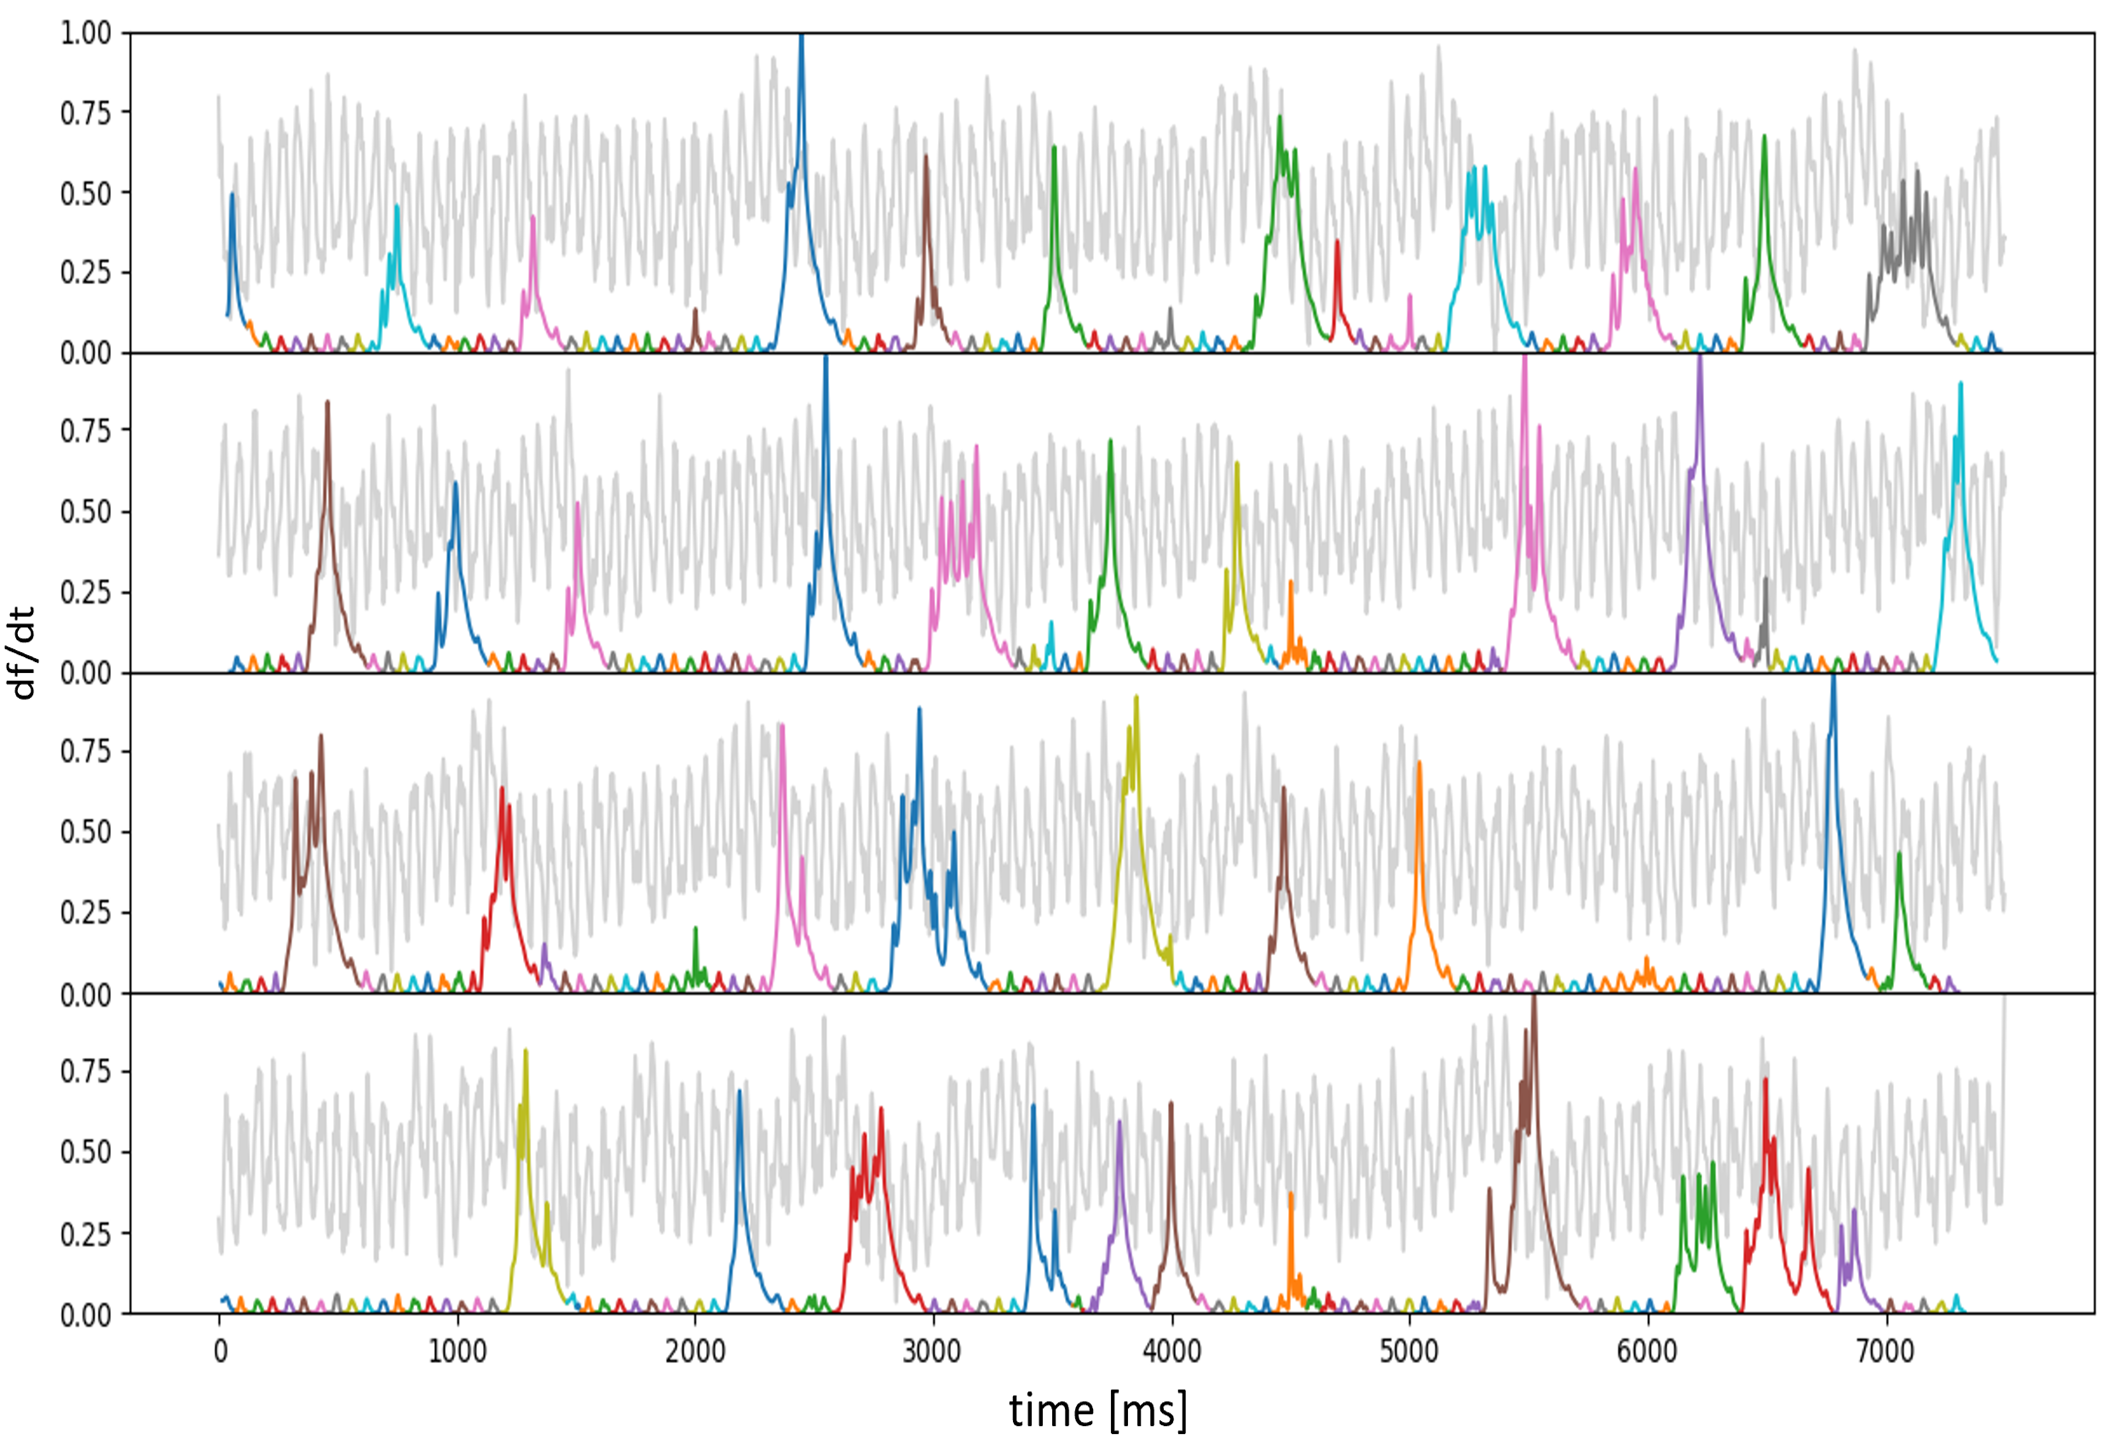
\includegraphics[width=\textwidth,height=\textheight,keepaspectratio]{Figures/slow_wave_segmentation}
\decoRule
\caption[Detected slow waves for a sample recording]{Detected slow waves for a sample recording at 1.8 \% isoflurane.\\ The depiction shows the results of the splitting procedure. Segments of the baseline-corrected mean percentage change that were identified as one event are represented in the same color. Note that the approach identifies events in a scale independent manner. Colors indicate segments of the df/f signal for a complete recording (GCaMP). The hemodynamic signal is plotted in the background in grey.}
\label{fig:slow_wave_segmentation}
\end{figure}

\label{Chapter4} % Change X to a consecutive number; for referencing this chapter elsewhere, use \ref{ChapterX}

%----------------------------------------------------------------------------------------
%	SECTION 1
%----------------------------------------------------------------------------------------
 The approach for the analysis of slow waves includes three steps: Detection of events, feature extraction using Optical Flow and Helmholtz Decomposition as well as dimension reduction by aggregation and the use of Autoencoders. Slow oscillations were detected in the df/f signal such that an event related analysis could be performed. Aggregated features were analysed quantitatively. Moreover individual waves were investigated qualitatively in more detail. This analysis includes several features such as the peak amplitudes and the directions of flow on one side as well as the vector fields on the other. The results are presented in this section.\\
 \begin{figure}[!htb]
 \centering
 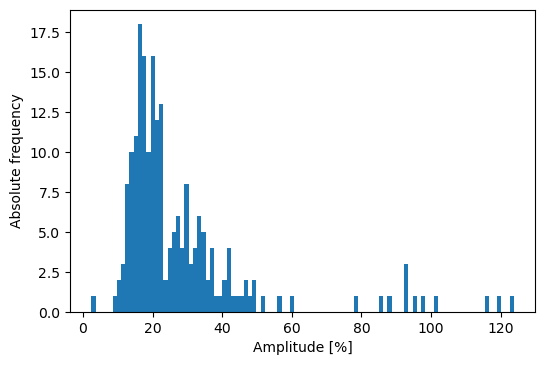
\includegraphics[width=\textwidth,height=\textheight,keepaspectratio]{Figures/selected_waves_distribution_of_peak_amplitude}
 \decoRule
 \caption[Distribution of the peak amplitude of detected waves]{Distribution of the peak amplitude of detected waves.\\The depiction shows the distribution of the peak amplitude of the selected slow waves after cleaning the dataset. Cleaning includes removal of instances that are highly correlated (r>.3) with the hemodynamic breathing signal. In addition, it comprises the removal of waves for which the peak activity of the mean percentage change in time is less than 5\% of the duration. Note that events with a peak amplitude of below 5\% are virtually absent.}
 \label{fig:selected_waves_distribution_of_peak_amplitude}
 \end{figure}
 Figure \ref{fig:slow_wave_segmentation} shows an example for the detection of slow waves for a sample recording (iso = 1.8\%). The procedure was found to yield segmentations that meet the human intuition for all stages of anaesthesia. Note that several of the depicted events are similar with respect to shape and size. Different types can be distinguished. Some events have a single peak while others have multiple ones and show longer up states. \\
 Note that a trend in the hemodynamic signal is related to the occurrence of large amplitude events: While the hemodynamic signal appears to increase before the occurrence of large amplitude events it drops during the respective neocortical slow wave. The latter arguably indicates effects of neurometabolic coupling and represents a BOLD response. The circumstance that a rise in the hemodynamic signal precedes neocortical slow waves could mean that higher blood oxygen levels promote the occurrence of runaway neural firing. \\
 Events for which the df/f signal correlates strongly with the hemodynamic signal were excluded from the further analysis. These events relate to large amplitude neocortical slow waves that have a good signal to noise ratio. It was found that the most interesting patterns are visible for these events. Waves with a peak amplitude below 5\% are virtually absent in the filtered dataset of slow waves. The dataset of large amplitude slow waves includes 204 samples from two animals and five experimental conditions. Figure \ref{fig:selected_waves_distribution_of_peak_amplitude} shows the distribution of peak amplitudes.\\
The activity of neurons is inhibited at higher dosages of isoflurane (Figure \ref{fig:typical_examples_and_peak_amplitudes}: B). This results in widespread quiescence for deep anaesthesia. Coherently it shows that the distribution of slow wave amplitudes decreases for higher levels of isoflurane. While neocortical slow waves occur with a peak amplitude of up to 120\% signal change they mostly rely around 20 \% for an isoflurane level of 2.6\%. \\
\begin{figure}[!htb]
\centering
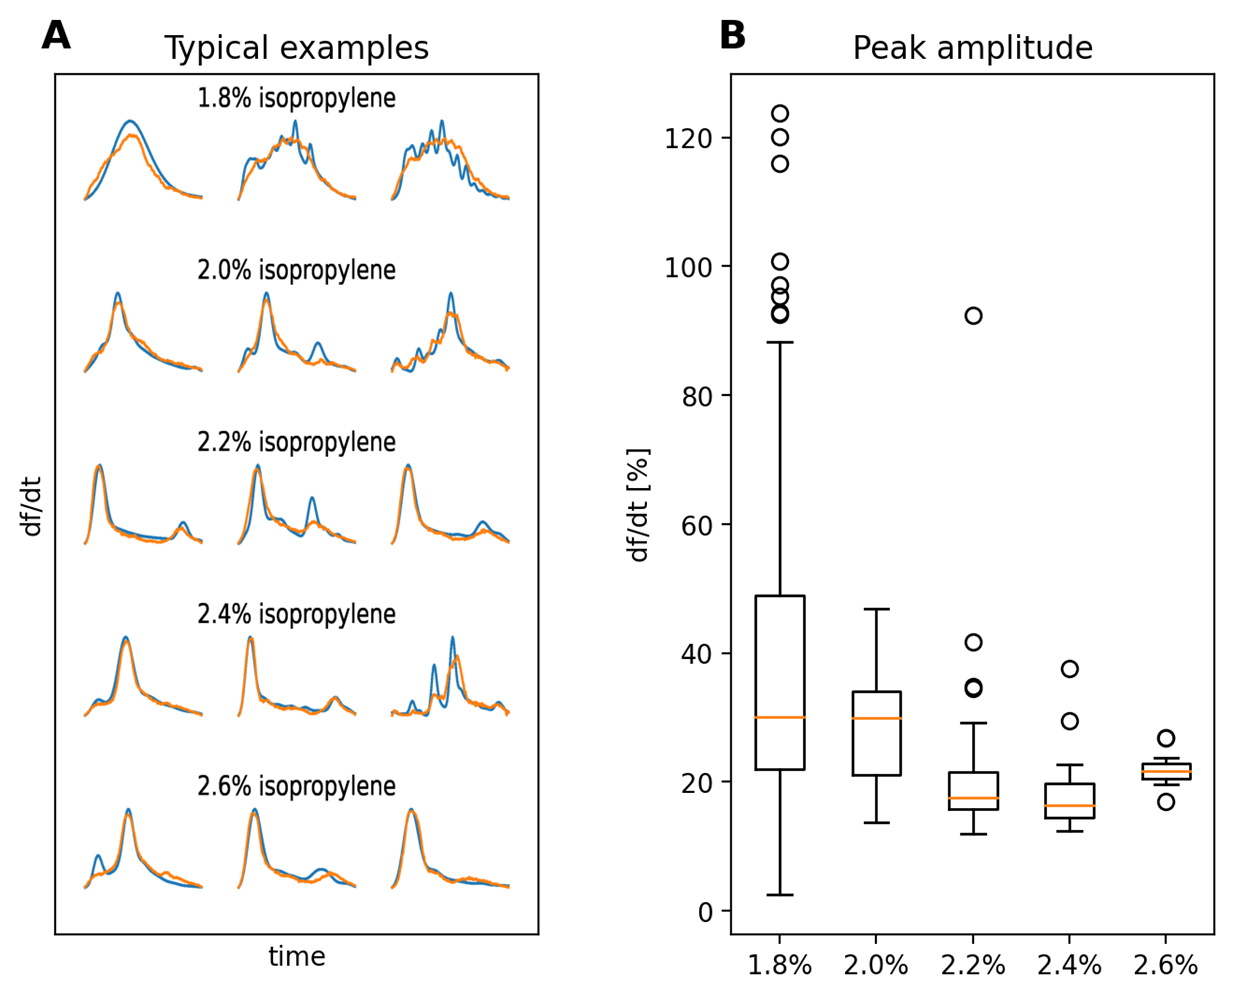
\includegraphics[width=\textwidth,height=\textheight,keepaspectratio]{Figures/typical_examples_and_peak_amplitudes}
\decoRule
\caption[Typical examples and peak amplitudes]{Typical examples and peak amplitudes.\\The depiction shows data for slow waves with a peak amplitude above 5\% that are only weakly correlated with the hemodynamic signal (r<.3). Panel A: Typical examples for slow-wave events during different stages of anesthesia. The mean signal change over time is indicated in blue while reconstructions of the Variational Autoencoder with fully connected layers are plotted in orange. Panel B: The distribution of the peak amplitudes of the mean signal over time for each slow wave per condition.}
\label{fig:typical_examples_and_peak_amplitudes}
\end{figure}
The shape of the events differs between conditions. Typical examples of the df/f signal and the reconstructions of the Autoencoder for the slow wave shape space are indicated by Figure \ref{fig:typical_examples_and_peak_amplitudes}:A. At 1.8\% isoflurane slow waves are present that have an extended up state and multiple peaks. Single peak waves and waves with two larger peaks are especially characteristic for 1.8\% and 2.0\% isoflurane. At higher levels of anesthesia another type can be observed that comprises of one major peak and a much smaller one that occurs subsequently. This type of neocortical slow wave arguably reflects synchrony between neural firing and breathing (see also \cite{tort2018parallel}). Its shape results from a major neocortical slow wave that is followed by a peak which is correlated with the breathing signal. While different types of neocortical slow waves occur preferably for specific concentrations of isoflurane each condition can be described as a composition of different types of events.\\
\begin{figure}[!htb]
\centering
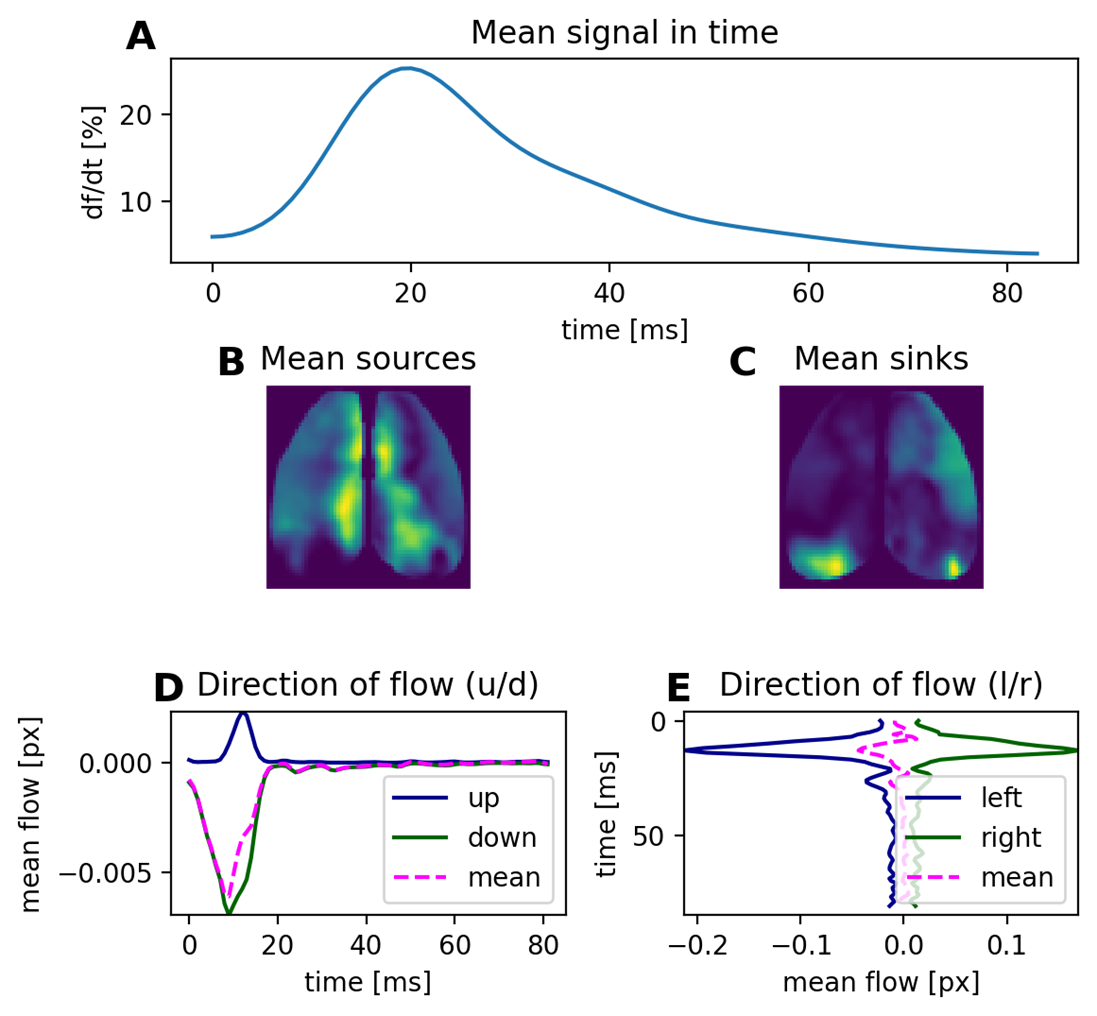
\includegraphics[width=\textwidth,height=\textheight,keepaspectratio]{Figures/percentage_change_direction_of_flow_and_sources_sinks}
\decoRule
\caption[A typical example with one peak]{A typical example with one peak.\\Percentage change, direction of flow and the distribution of sources and sinks. Panel A shows the mean percentage change in time. Panel B illustrates the mean sources and sinks distribution in space and Panel C illustrates the mean sinks distribution respectively. Note that the brain regions that act as sources are not identical with the regions that act as sinks which supports the idea of a sender-receiver pattern. Panels D and E indicate the direction of flow in vertical direction (up/down) and horizontal direction (leftwards/rightwards) respectively.}
\label{fig:percentage_change_direction_of_flow_and_sources_sinks}
\end{figure}
A general distinction of the spread of neural signals can be made for bottom up and top down flow. In the mouse cortex, bottom up flow can originate from auditory and visual areas in the occipital lobe as well as retrosplenial dysgranular cortex (RSD) which contains neural populations that code for places and is thought to integrate thalamic, hippocampal, and neocortical information \parencite{milczarek2018spatial, van1992connections}. It shows that there is a trend towards lower levels of bottom up flow for higher levels of isoflurane. However this trend is not significant (see Figure\ref{fig:direction_per_isoflourane}).\\
\begin{figure}[!htb]
\centering
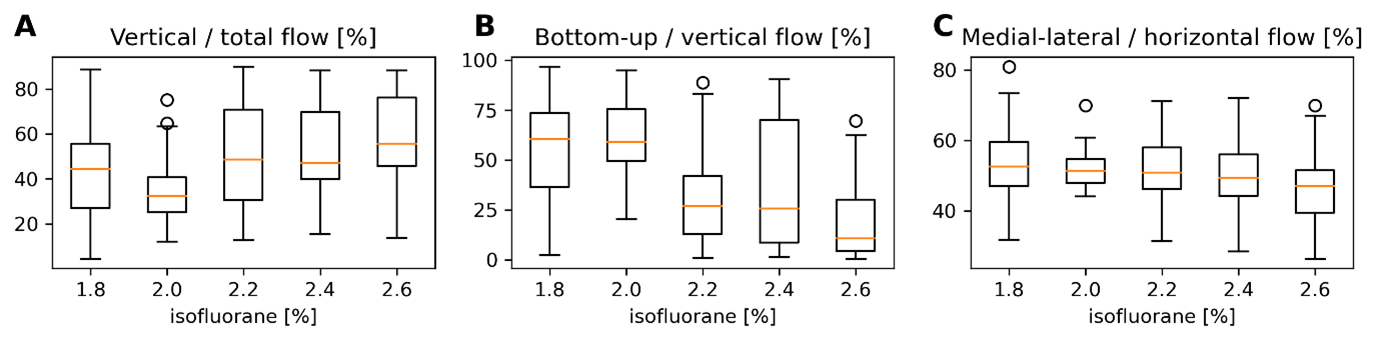
\includegraphics[width=\textwidth,height=\textheight,keepaspectratio]{Figures/direction_per_isoflourane}
\decoRule
\caption[Direction of flow for different levels of isoflurane]{The direction of flow for different levels of isoflurane.\\Panel A: Vertical flow (the sum of the absolute Y-components of the vectors of the flow field) as a proportion of total flow. Panel B: Bottom-up flow as a proportion of vertical flow. Panel C: Medial to lateral flow as a proportion of horizontal flow (the sum of absolute X-components of the vectors of the flow field). Note that the flow component retrieved via Helmholtz  of the Optical-Flow are the basis for the aggregated data displayed here.}
\label{fig:direction_per_isoflourane}
\end{figure}
The vector fields of the flow component can be evaluated qualitatively. Figure \ref{fig:vector_field_flow_component} illustrates the relationship between the df/f signal, the field strength and the vector field of flow for an example with a single peak where downwards and leftwards flow can be observed in the left hemisphere. In the right hemisphere mainly right-downwards flow occurs. However, at peak activity rightwards flow dominates. The dynamics of the event are also illustrated by Figure \ref{fig:percentage_change_direction_of_flow_and_sources_sinks}. The aggregations reflect the flow of the left hemisphere. Here the distribution of sources and sinks is plotted as well. Areas on the medial axis act as the main sources while visual areas act as sinks. The direction of flow and the distribution of sources and sinks characterize neocortical slow waves.\\
\begin{figure}[!htb]
\centering
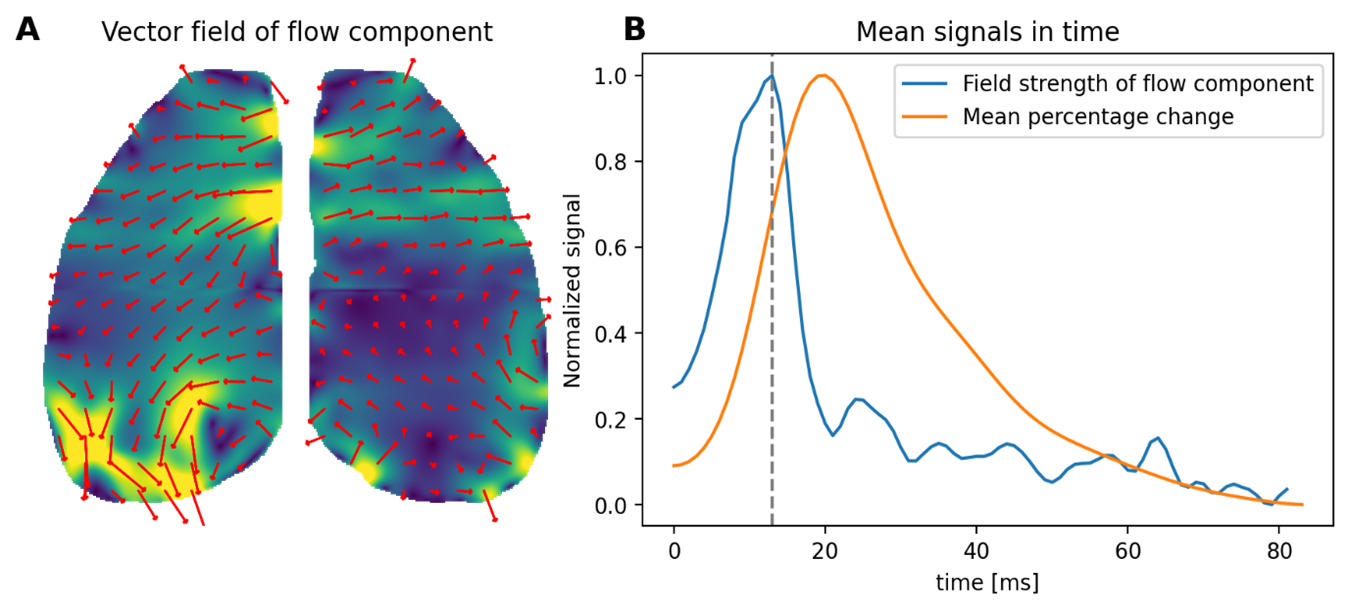
\includegraphics[width=\textwidth,height=\textheight,keepaspectratio]{Figures/vector_field_flow_component}
\decoRule
\caption[A sample vector field and field strength of flow in time.]{A sample vector field and field strength of flow in time.\\ The depiction shows a vector field for a slow-wave event at 1.8\% isoflurane alongside the mean percentage change and mean flow in time. Panel A: The vector field representation of the flow component. The field strength is plotted in the background. Panel B: The mean percentage change in time and the mean field strength of the flow component. Note that the signals are not to scale. The time of the depicted frame is marked by a vertical dotted line. Left-downwards flow shows for the left hemisphere.}
\label{fig:vector_field_flow_component}
\end{figure}
It is to mention that the spatial distribution of sources does not directly compare with the mean activity in space as measured by the df/f signal of an event. The temporal integral of the df/f signal does not reflect the distribution of sources as sources indicate focal areas of brightness increase. While the mean across all frames of the df/f signal can show little spatial variations the mean of the sources distributions reveals focal area of increasing neural activity (Figure \ref{fig:sources_are_not_mean_signal}).\\
\begin{figure}[!htb]
\centering
\includegraphics[width=\textwidth,height=\textheight,keepaspectratio]{Figures/sources_are_not_mean_signal}
\decoRule
\caption[The temporal mean of the df/f signal and the sources]{The temporal mean of the df/f signal and the sources.\\ The depiction illustrates that the temporal mean over all frames showing the df/f signal is highly dissimilar from the temporal mean of the sources for the same period. This shows the benefits of Helmholtz Decompositon applied on Dense Optical Flow. The approach allows to reduce dynamical changes of neural activity that occur during slow waves to a lower dimensional representation that reflects functionally connected regions.}
\label{fig:sources_are_not_mean_signal}
\end{figure}
Neocortical slow waves can incorporate several oscillations (see section \ref{working_definition}). In addition it can be assumed that even events with a single peak can incorporate several subsegments for which different areas act as sources or sinks and different patterns occur in the flow. To test this assumption slow waves were split into subsegments based on the local minima in the distribution of the sources. Figure \ref{fig:slow_wave_subsegements} illustrates the results. During different stages of the slow wave distinct areas represent the sources. It shows that this distribution can be distinguished into a lateral cluster that includes somatosensory areas (e.g. segment onset at 21ms) and a medial cluster that includes regions on the medial axis from frontal to occipital cortex (e.g. the last segment). These findings represent first evidence that different stages of slow waves exist in events that show only one peak in the temporal mean of the df/f signal. As the strength of sources during downstream periods is weaker, they are however more prone to artifacts in the contrast (see also \ref{processing_pipeline}). More research is required to systematically study the events that occur during different stages of neocortical slow waves.\\
\begin{figure}[!htb]
\centering
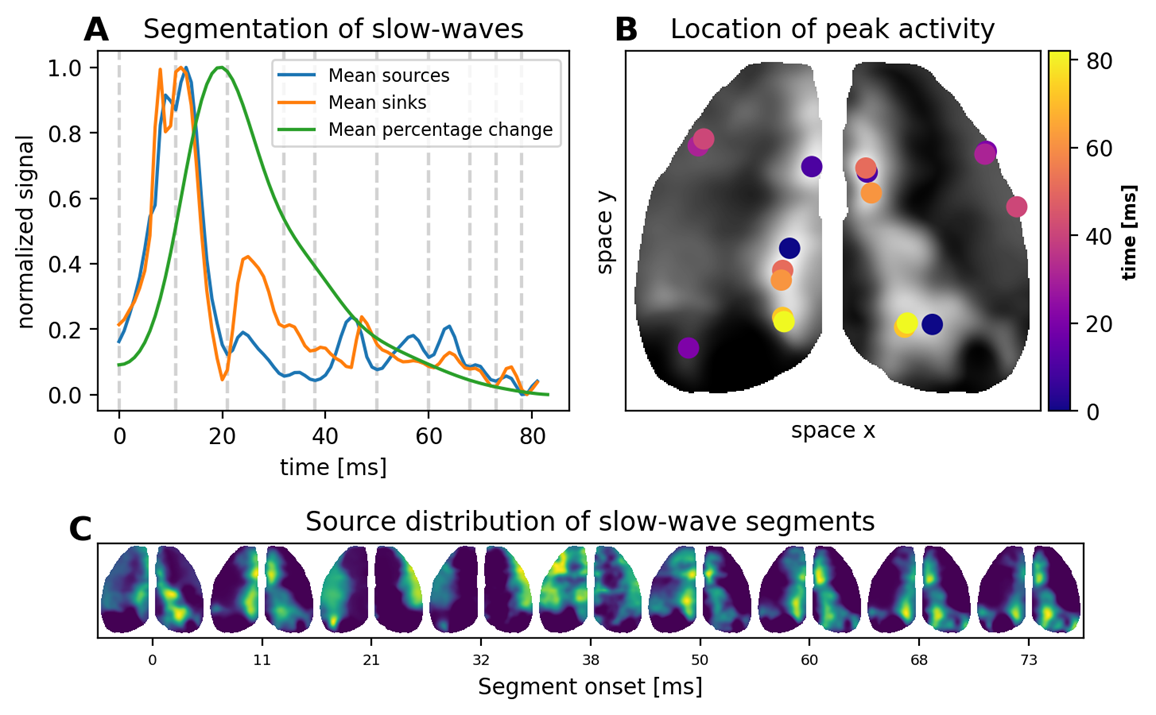
\includegraphics[width=\textwidth,height=\textheight,keepaspectratio]{Figures/slow_wave_subsegements}
\decoRule
\caption[Slow wave subsegments]{Slow wave subsegments.\\The depiction illustrates the procedure of splitting a slow wave into subsegments using the mean sources distribution. Panel A: The mean signal in time for the sources and sinks alongside the mean percentage change. Slow-wave segments are determined using local minima in the mean sources signal in time. Gray dotted lines indicate the onset and offset of each segment. Panel B: The location of peak activity. Panel B shows the location of maximal activity for the mean source signal in space of each subsegment (see Panel C). Note that the time of segment-onset is indicated by different colours. Each dot corresponds to the segments identified in A and the mean source signal in space in C. Panel C: The temporal mean of the source signal in space for the identified slow-wave segments. Note that the depictions normalized before a colormap was applied to increase the contrast. Yellow tones relate to higher values.}
\label{fig:slow_wave_subsegements}
\end{figure}




\section{Reconstruction manifolds and latent space distributions}
Several different types of neocortical slow waves can be discearned Intuitively based on the shape of the temporal mean of the respective df/f signal. Moreover the direction of flow and the distribution of sources differs between events. Besides it was argued that different compositions of events are characteristic for specific levels of anaesthesia. Autoencoders can be used for dimension reduction and represent a tool that allows to vizualize the complex dynamics of slow wave anaesthesia. Three models were implementes. In the following the results of these models are presented that indicate (1) the distribution of several features in latent space and (2) can be used to compute manifolds of reconstructions. Autoencoders can help in revealing the complex dynamic of slow waves.\\
\begin{figure}[!htb]
\centering
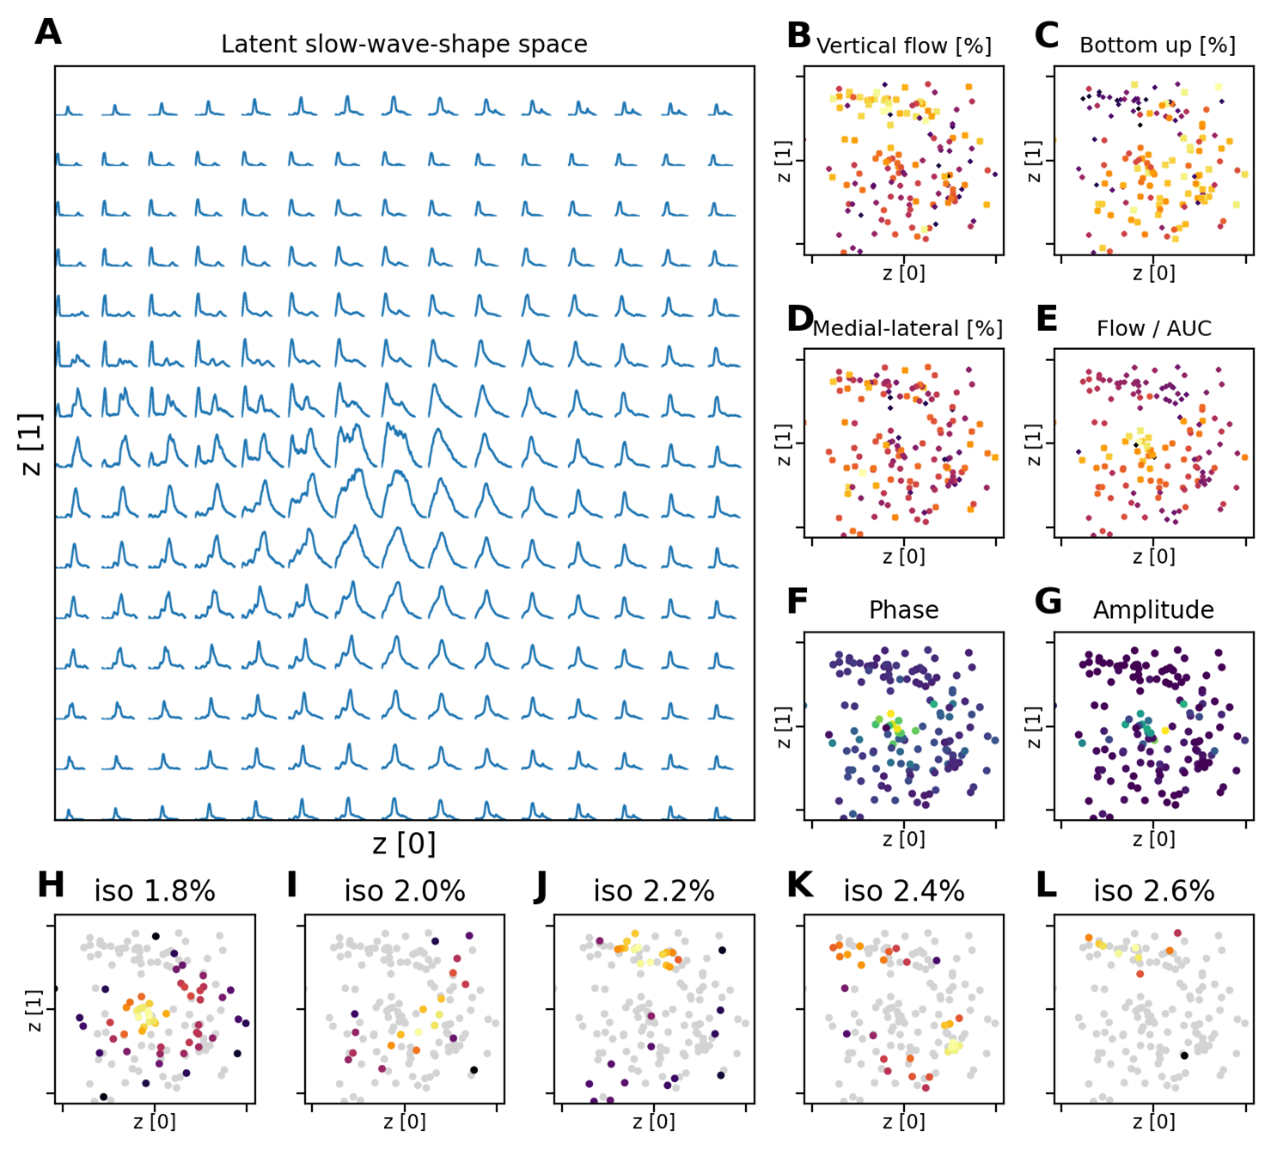
\includegraphics[width=\textwidth,height=\textheight,keepaspectratio]{Figures/slow_wave_shape_space}
\decoRule
\caption[Latent slow wave shape space]{Latent slow wave shape space.\\Note that events with peak-amplitude below 5\% signal change and a high correlation with the hemodynamic breathing signal (r>.3) were excluded from the analysis. Panel A: Latent slow wave shape space. The panel shows a manifold of decodings for different combinations of the activation of the latent-layer neurons z[0] and z[1]. Note that the latent-layer activations are chosen from an evenly spaced grid. The minimal and maximal values for each dimension of this grid are chosen as $\bar{z}\pm\delta\left(z\right)$ with z = encoder(x). The decodings of the vectors are scaled according to the predictions of the width and height and plotted using a square root scale to ensure good visibility of small magnitude events. Panel B: The proportion of the absolute vertical flow as a fraction of the absolute flow during each wave. Panel C: The proportion of bottom-up flow as a fraction of the vertical flow. Panel D: The fraction of medial-lateral flow as a fraction of horizontal flow. Panel E: The ratio between mean absolute flow and the area under the curve of the mean percentage change for each wave. Panel F: The phase/duration of each event. Panel G: The distribution of the amplitude (peak of mean percentage change) for each of the events. Panels H-L: The distribution of samples in latent slow wave shape space.}
\label{fig:slow_wave_shape_space}
\end{figure}
The first Autoencoder is a simple model that employs a MLP as encoder and decoder. As the input vector has few entries, fully connected layers can be used without compromising on the computational cost. The model reveals the distibution of several features in slow wave shape space. For the analysis presented here the Autoencoder was trained on the df/f signal for each event. Then the whole dataset was mapped onto the latent space. This space is spanned by the activation of the latent layer neurons z[0] and z[1]. Several properties of each event can be visualized. Distinct regions in the low dimensional representation of neocortical slow waves relate to different types of waves. As a variational Autoencoder was used the latent space is comparatatively densely populated. This means one may interpolate between events. Activations of the latent layer neurons can be chosen from an evenly spaced grid such that most of the data is covered. Using the decoder model the respective reconstructions can be retrieved. Figure \ref{fig:slow_wave_shape_space} indicates this manifold alongside the distribution of several properties in latent slow wave shape space.\\
In general larger waves are mapped to the center while smaller waves rely in the periphery: The phase and amplitude is higher for the respective samples (\ref{fig:slow_wave_shape_space}:F-G). The samples in the center region also have stonger flow as measured by the area under the df/f curve. Samples from the different experimental conditions are unevenly distributed in latent slow wave shape space. Most samples an isoflurane level of 1.8\% rely within the center and represent events with multiple peaks and extend upstate periods. At 2\% more samples rely further to the lower right. These areas correspond to reconstructions that mainly represent neocortical slow waves with one major peak. For higher levels of isoflurane a cluster exists in the upper right. This cluster arguably corresponds to waves where the smaller peak corresponds to an oscillation that is synchronous with the breathing signal. These samples have stronger vertical flow (as compared to horizontal flow) and less bottom-up flow as compared to top-down flow (\ref{fig:slow_wave_shape_space}:B-D). Other samples of the very deep anaesthesia conditions (iso>2\%) are mapped to the periphery close to the lower and right border of the displayed subspace. This indicates a general shift from longer lasting up states with more oscillations to less dynamical states where smaller waves typically have only one peak.\\
\begin{figure}[!htb]
\centering
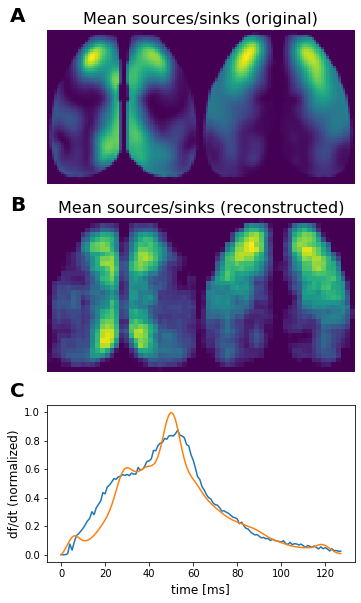
\includegraphics[width=\textwidth,height=\textheight,keepaspectratio]{Figures/reconstructions_example_mixed_input}
\decoRule
\caption[Examples for reconstructions of the mixed input model]{Examples for reconstructions of the mixed input model.\\ Panel A: The distribution of sources (left) and sinks (right). Panel B: The reconstructions of the image shown in A. Panel C: The respective df/f signal and the reconstructed signal.}
\label{fig:reconstructions_example_mixed_input}
\end{figure}
\begin{figure}[!htb]
\centering
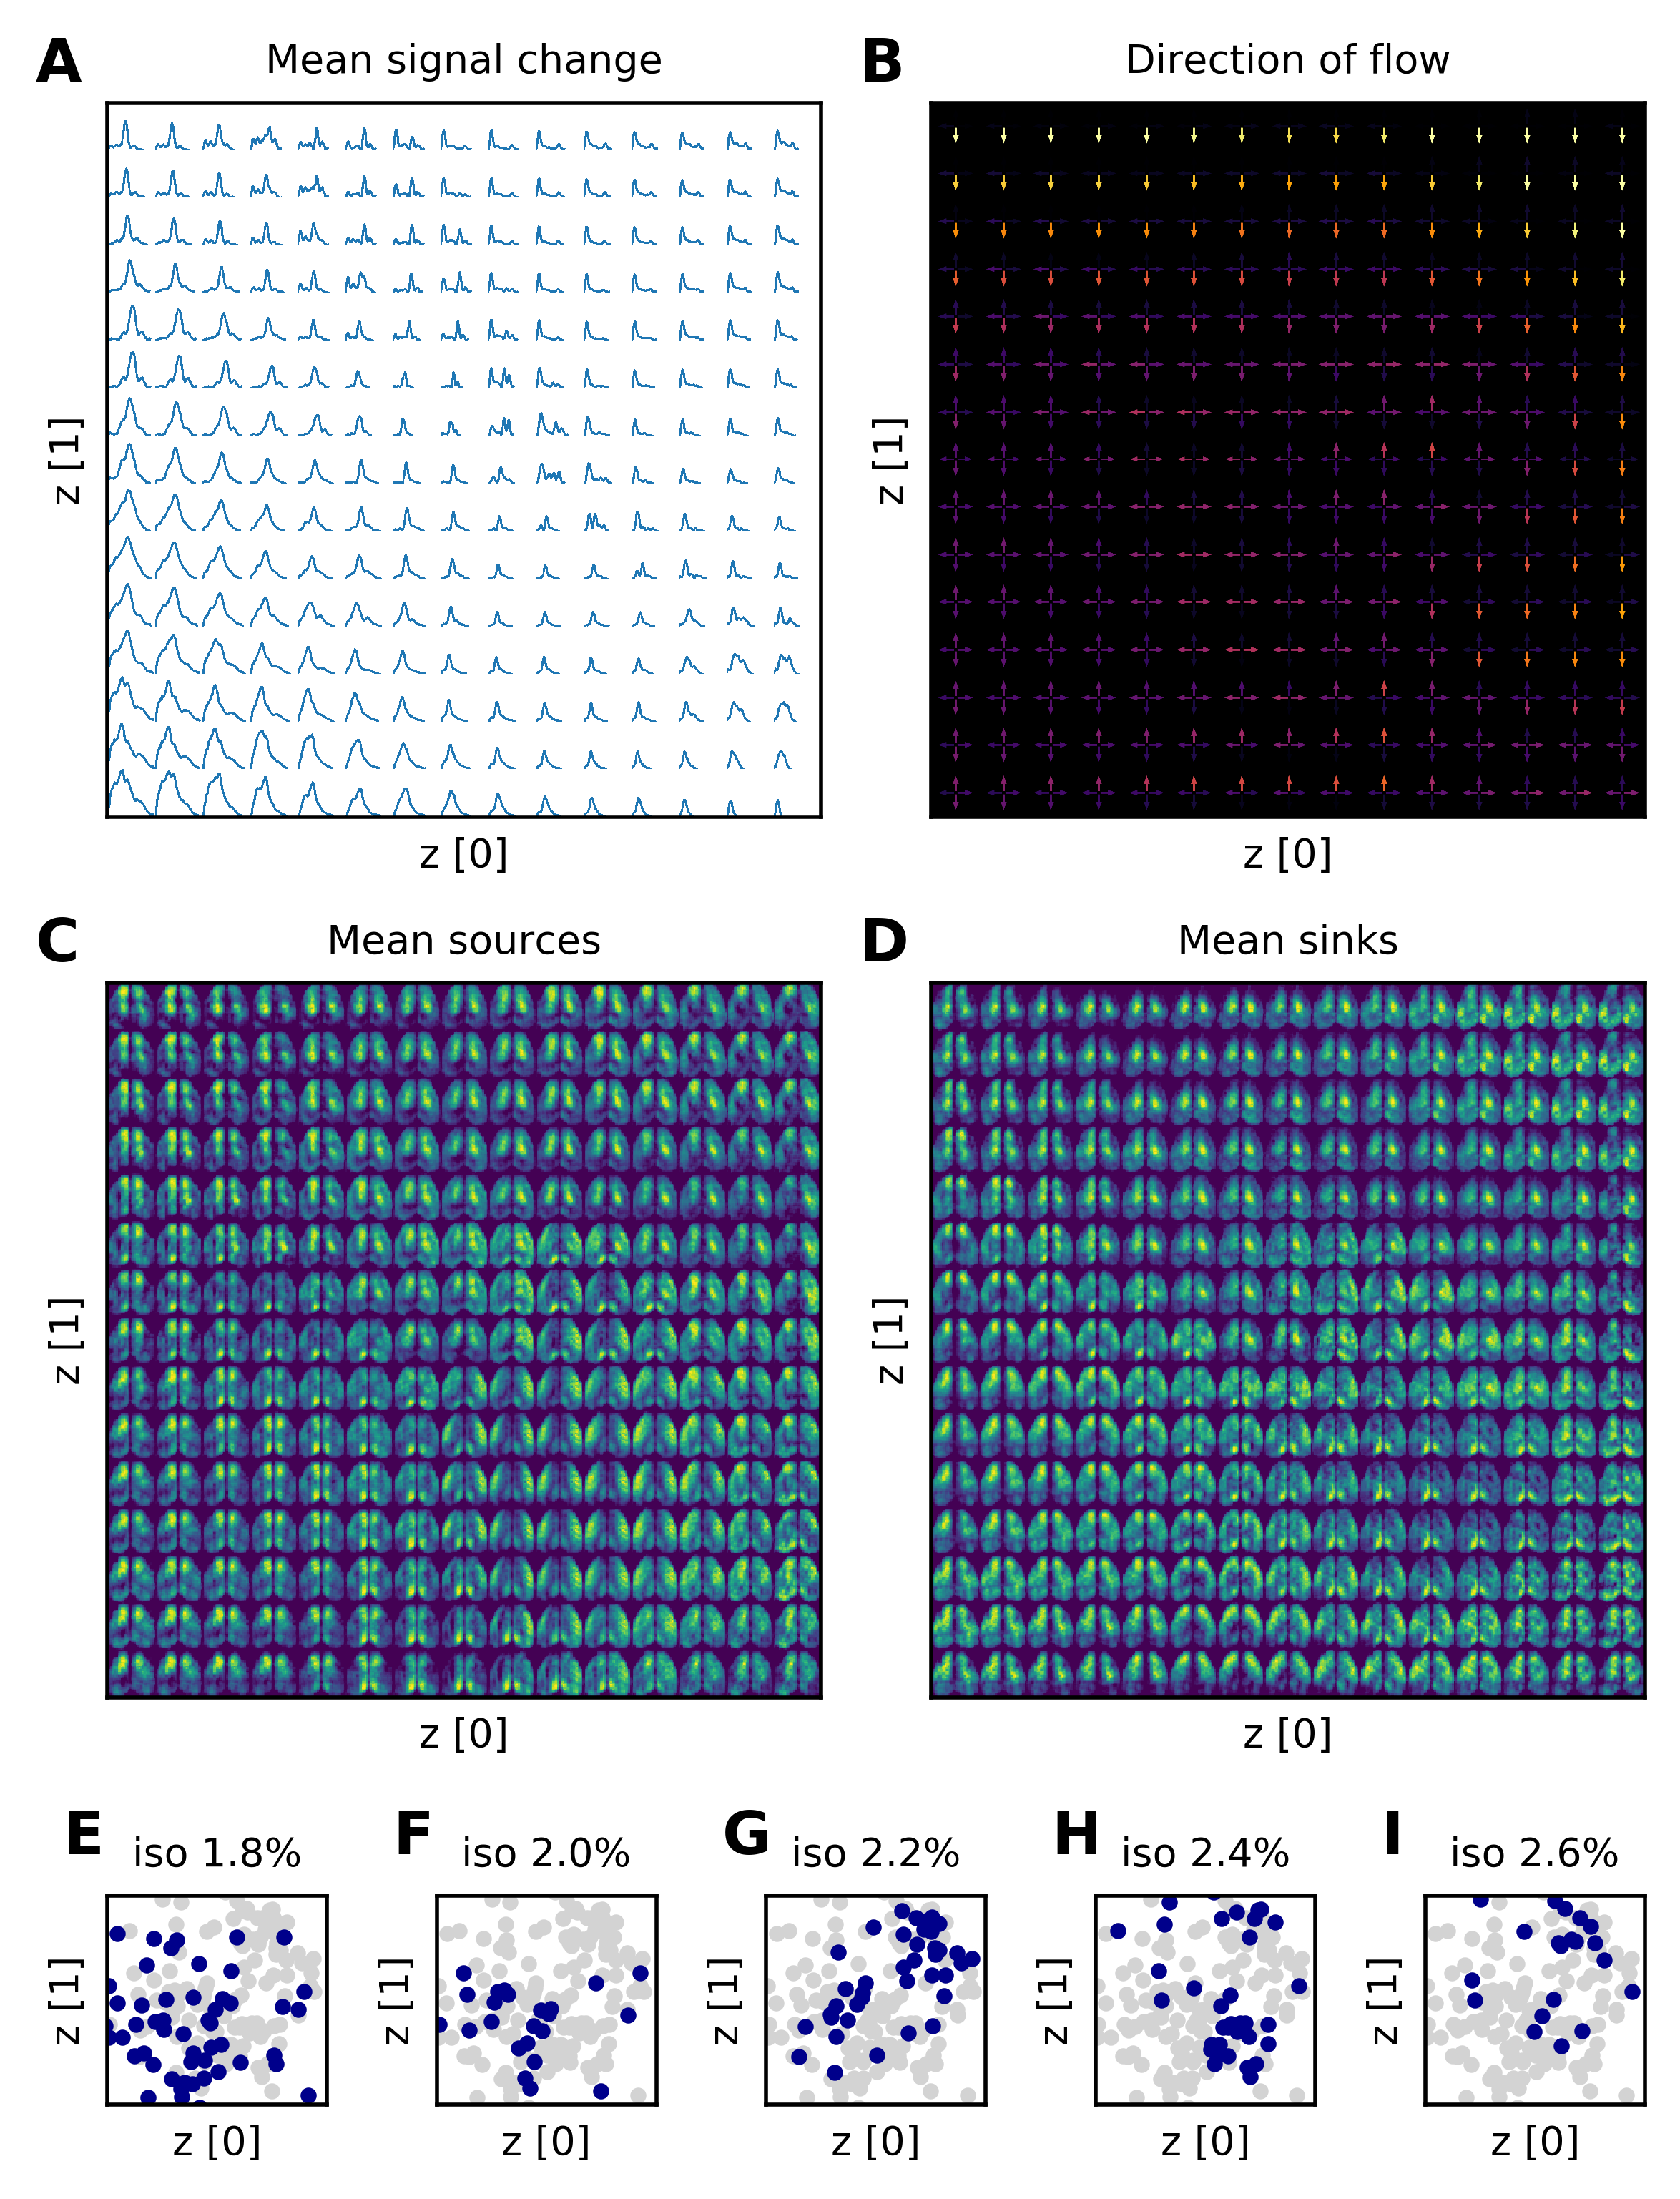
\includegraphics[width=\textwidth,height=\textheight,keepaspectratio]{Figures/latent_slow_wave_space}
\decoRule
\caption[Latent slow wave space]{Latent slow wave space\\The depiction shows the results of for the mixed input model. Note that events with peak-amplitude below 5\% signal change and a high correlation with the hemodynamic breathing signal (r>.3) were excluded from the analysis. Panel A: Slow wave shape space. The panel shows the reconstructions of the df/f signal for the mixed input model. Duration and amplitude are square root scaled. Panel B: The direction of flow. Arrows indicate the reconstructions for the ratio of flow for each event. Note that upwards flow dominates in the lower center, flow occurs in all directions rather evenly in the middle left portion while downwards flow dominates for events in the upper right area. Panel C and D: The reconstructions of the sources and sinks. Note that differences in the distribution of sources and sinks are most strongly pronounced in the lower central part. Panel E-I: The distribution of samples of different experimental conditions in latent slow wave space. Note that the density of the distribution for overlapping points is color-coded. All samples that do not belong to the respective condition are plotted in grey.}
\label{fig:latent_slow_wave_space}
\end{figure}
The second Autoencoder is used in the same way as explained for the previous one. However it is trained on more features that arguably make up the most important characteristics of neocortical slow waves: The shape of the df/f signal alongside the duration and amplitude, the ratio between flow in different directions as well as the distribution of sources and the distribution of sinks. Hence latent slow wave space allows for a more complete distinction of neocortical slow waves that most importantluy includes the distribution of focal areas of recurrent activity. The performance of the reconstructions is indicated by Figure \ref{fig:reconstructions_example_mixed_input}. Although only a two dimensional latent space was used an acceptable reconstruction was achieved for all included features.\\
The arrangement of slow wave shapes in the latent space of the second Autoencoder differs from the first one. Here large amplitude waves with multiple peaks are mapped to the lower left corner. Large single peak waves correspond to an area between the center and the lower right corner. Small waves that can include a second peak rely above the diagonal in the upper right area. The distribution of sources reveals that the shape of neocortical slow waves is related to focal areas of recurrent activity. Sources in frontal areas are present for small waves that exist mainly during very deep anaesthesia. This type of small waves is characterized by downwards flow.\\
The manifold of sources and sinks provides further information regarding the nature of larger waves. Neocortical slow waves that are mapped to a region to the lower right of the center have sources in areas of the brain that arguably relate to the barrel fields. In contrast, large waves that potentially include multiple peaks have sources either in frontal areas or in a medial band that includes the RSD. Especially for the latter kind of events sinks reside in areas different from the sources and upwards flow dominates. However there are areas as well where the horizontal flow is strong. Visual inspection of the vector field animations shows that this kind of waves includes upwards flow that is stongest in medial portions in early stages of the events while medial lateral flow occurs mainly in frontal areas in later periods. Large neocortical slow waves can exist in the form of medial axis events with bottom up flow and as frontal events that sometimes exhibit pronounced downwards flow. \\
The latent space mappings described above illustrate a complex topology of neocortical slow waves. However, a third Autoencoder was used to analyse the exact temporal dynamics of upwards and downwards flow in relation to the df/f signal. Here the normalized df/f signal as well as a signal for upwards and downwards flow were used. It shows that a peak in vertical flow occurs during the first major rising phase of neocortical slow waves. Latent space reconstructions reveal events where upwards flow is stonger than downwards flow and waves where the opposite is the case. In the center left of the reconstruction manifold one may find events with multiple peaks where downwards flow occurs during the first rising phase while upwards flow is stronger during the rise of a second peak.\\

\begin{figure}[!htb]
\centering
\includegraphics[width=\textwidth,height=\textheight,keepaspectratio]{Figures/latent_flow_space}
\decoRule
\caption[Latent slow wave flow space]{Latent slow wave flow space\\ The depiction illustrates the relationship between the signal change of the fluorescence signal (df/f) and periods of upwards and downwards flow. Autoencoder 3 was used to compute the mappings to latent space and decodings using an evenly spaced grid that covers the majority of points. Panel A: A reconstruction manifold where blue lines relate to the df/f signal. Green lines indicate the strength of upwards flow, as measured by the mean Y component per frame, for periods where this measure is positive. Analogously orange relates to downwards flow. Note that the periods where the vertical flow is most pronounced coincide with the rising phase of the df/f signal. For some events several peaks in flow occur that correspond to several oscillations in the df/f signal. Moreover, the preferred direction of flow is not necessarily the same during these subsegments. Panel B-F: The distribution of samples of different experimental conditions in latent slow wave flow space. Note that the density of the distribution for overlapping points is color-coded. All samples that do not belong to the respective condition are plotted in grey.}
\label{fig:latent_flow_space}
\end{figure}
%-----------------------------------
%	SUBSECTION 2
%-----------------------------------

\section{The relationship of the breathing signal (405nm) and the GCaMP signal (460nm)}
In the main analysis presented here, events were excluded for which a strong correlation between the GCaMP signal and the breathing signal exists (r>.3). This was done to exclude oscillations from the analysis that result from hemodynamic effects. The impact on the signal of large amplitude events was found to be negligible. However it showed, that small amplitude events can occur phase locked to a peak that correlates with breathing: A cluster of small amplitude events that include a second peak represents this kind of slow waves.\\
\begin{figure}[!htb]
\centering
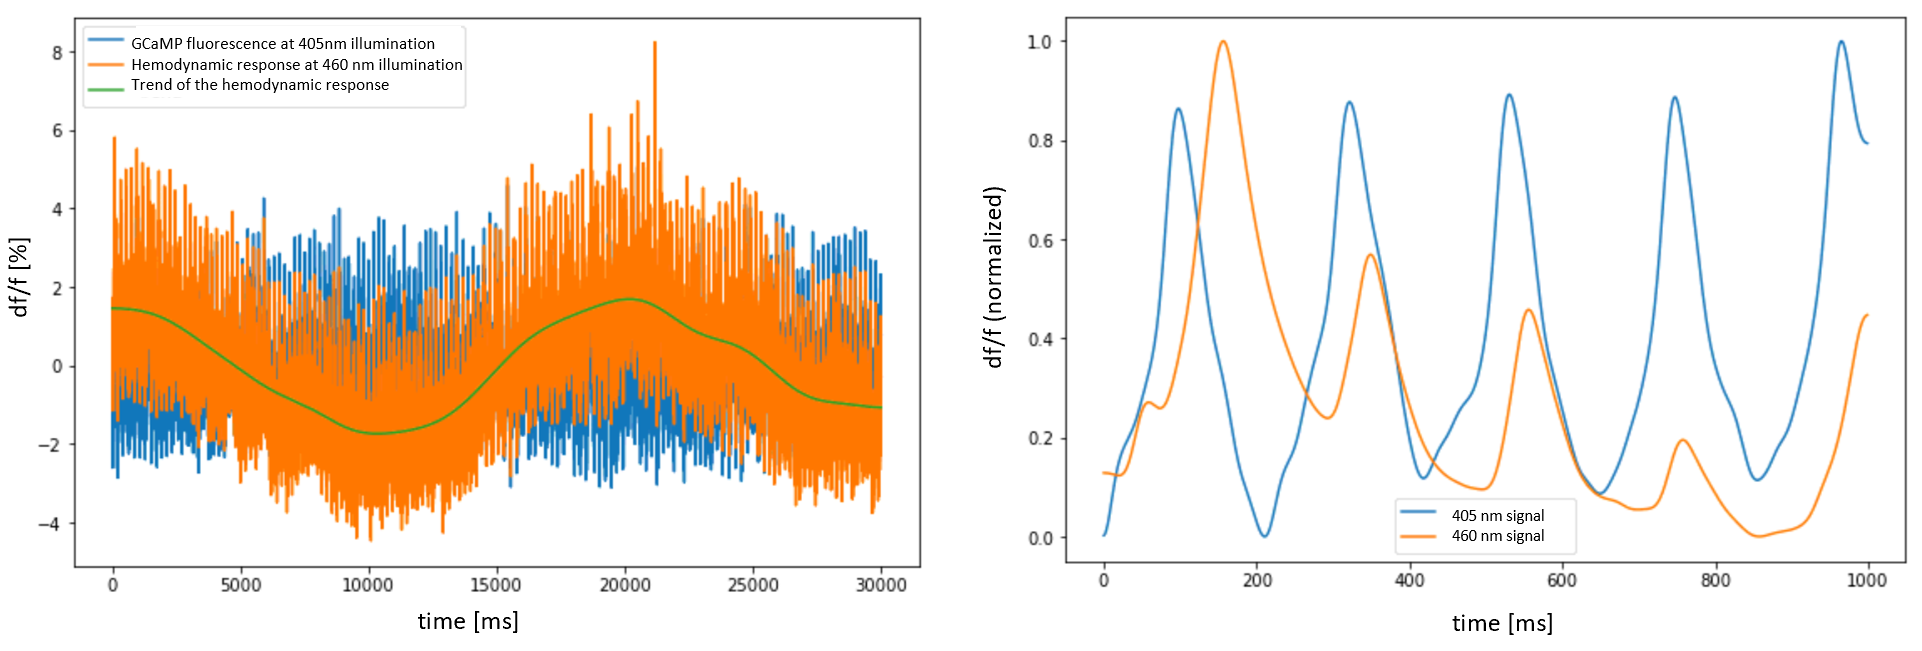
\includegraphics[width=\textwidth,height=\textheight,keepaspectratio]{Figures/hemodynamic_signal}
\decoRule
\caption[The relationship between breathing and the GCaMP signal]{The relationship between breathing and the GCaMP signal\\ The depiction illustrates the preprocessed signals for breathing (405nm) and the GCaMP signal (460nm). Left: The spatial mean of the df/f signal for both signals and a recording at 2.4\% isoflurane. Right: A close up for a 10s period. Note that several oscillations are aligned but the GCaMP signal differs in amplitude in contrast to the breathing signal.}
\label{fig:hemodynamic_signal}
\end{figure}
The anaysis of small amplitude events reveals another pattern. GCaMP waves of variable amplitudes are coaligned with the breathing signal at 405nm for some recordings and high levels of anaesthesia. If the osciallation in the GCaMP signal was only an artifact one would not expect the amplitude to vary independant from the breathing signal where variations are negligible (see \ref{fig:hemodynamic_signal}). It was also found that the spatial distribution of GCaMP flourosence at peak activity does not reflect the one of the breathing signal at 405nm. Both indicates that highly correlated GCaMP oscillations exist that cooccur with the breathing signal and manifest as a superimposed peak in the spatial mean of the df/f signal.\\
The mixed input autoencoder was trained on events with a high correlation between the breathing signal and the GCaMP signal to further assess the relationship. It shows that sources exist in various regions for different events. However, a cluster of events exists where sources occur in regions of the brain that arguably relate to the barrel fields (see \ref{fig:latent_slow_wave_space_small_waves}). Further analysis shows that the events that relate to this cluster have a typical peak amplitude between 5\% and 10\%. The barrel fields are known to process sensory information from the whiskers. A potential explanation is that this type of breathing related oscillation at 460nm relates to perceptual effects of proprioception.
\begin{figure}[!htb]
\centering
\includegraphics[width=\textwidth,height=\textheight,keepaspectratio]{Figures/latent_slow_wave_space_small_waves}
\decoRule
\caption[Latent slow waves space for breathing correlated oscillations]{Latent slow waves space for breathing correlated oscillations.\\The depiction shows the latent space distibutions for the mixed input autoencoder that was trained on oscillations in the GCaMP signal that are substantially correlated with the breathing signal at 405nm. Panel A: Manifold of normalized reconstructions of the df/f signal. Panel B: The ratio of flow. Panel C: The distribution of sources. Panel D: The distribution of sinks. Panels E-F: The distribution of examples for the experimental conditions in latent space. Note that a cluster of waves exist in the lower left corner where sources rely in lateral areas.}
\label{fig:latent_slow_wave_space_small_waves}
\end{figure}
